\chapter{Introduction}
The concept of provenance (from the latin \textit{provenio}, ``to
come forth''), has been around for a long time~\cite{Bearman1985}.
It has been used in many other fields outside of computer science,
primarily that of art and antiques, where the provenance of a piece
is used as a guide to authenticity and quality. It has also been
used in the field of accounting in relation to auditing as well as
in databases, linking tuples in a query output to the reasons they
exist.

In this paper, provenance is a form of metadata representing the
lineage of a dataset or digital object. This is similar to the
information stored in a version control system but
goes beyond versions and authorship 
to capture a wider range of lineage data. 
Provenance makes it possible to identify and trace what other pieces
of information and activities have led to a digital object being in its
current state.

Large amounts of system-level, \textit{observational} provenance can be captured automatically and inexpensively, as in PASS~\cite{Macko2011,180755}. 
User-level provenance, however, depends more on the specific application,
as in Burrito~\cite{Guo2012}, an application created to help automate the more tedious aspects of experiment organisation and note taking. It captures the user activities such as web history, command line arguments and modified files, whilst allowing the user to annotate and view these activities at any time. The captured provenance then supports exploration of a single element. The user can view the provenance of an outputted provenance graph to see versions of the graph as well as the commands and input files used to create it. This allowed users to freely experiment, tweaking arguments and input to create different graphs, knowing that, at any point, they could explore the provenance to find what created any versions of a graph.

Burrito, and similar early interfaces, stored provenance information in a variety flat file formats. Since 2013, the PROV specification~\cite{primer2013} provides a standard generic model for provenance, with well-defined domain-specific extension points and a number of serialisations (RDF, XML, JSON, PROV-N).
%
PROV statements express ``\emph{descriptions of the entities and activities involved in producing and delivering or otherwise influencing a given object}'' and they are underpinned by three main concepts illustrated in Fig.~\ref{fig:key-concepts}:
(i) Entities: Physical, digital, conceptual objects, (ii) Activities: An element that causes an entity to come into existence, and (iii) Agents: Someone or something that can be assigned responsibility for an activity taking place.

\begin{figure}[h]
	\centering
	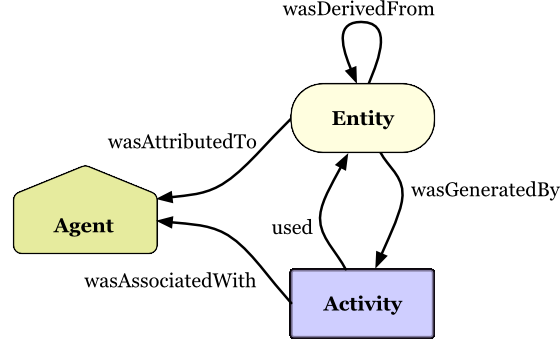
\includegraphics[width=0.4\linewidth]{key-concepts}
	\caption{Key Concepts and relationships from the PROV standard displayed in a labelled acyclic graph.}
	\label{fig:key-concepts}
\end{figure}

Provenance data, especially of the observational, low-level kind, quickly grows in size. Whilst the examples in this paper only show graphs with a small number of nodes, a provenance file can readily grow to millions of nodes. Because provenance stores historical data without summarisation, its grows monotonically over time. The speed of this increase is directly related to the granularity that the captured provenance. So, for example, capturing user actions typically makes the increase slower than is the case for operating system actions. In both cases, however, handling these large graphs causes both technical and usability issues. 

From a technical stand point it becomes resource intensive to scan a provenance file and display a visualisation of it, more so if the application reading the file runs analysis or summarisation of the data. 
%
Even more critically, from a usability perspective, it quickly becomes difficult for a user to interpret and explore such a large amount of information. The question then becomes how to ensure 
%% it is far more than cognitive load so I have altered this -- we can discuss it
%% the cognitive load on 
users can readily understand, explore and find the information they want from a graph. 
We build on research in both provenance~\cite{Seltzer2011, Borkin2013} 
and large scale graphs~\cite{Schaffer1996, Abello2006} 
to tackle this problem by simplifying graphs.
We describe our approach as \emph{clustering}, meaning that we combine multiple nodes into a single node.
This means that there are fewer nodes on the screen, with new combination concepts.

Notable amongst prior attempts at adaptive visualization of provenance graphs is the MapOrbiter~\cite{Macko2011a}, which is based on \textit{semantic zoom} and applies primarily to low-level system provenance, like PASS~\cite{Macko2011}.  One limitation of the approach is that the \textit{semantic} aspect assumes a priori knowledge of the type of processes that appear in the provenance trace,  and of their hierarchical relationships.

Figures~\ref{fig:fitness-ungrouped} and~\ref{fig:fitness-grouped} illustrate our approach
for an entity \texttt{Report}, written by \texttt{Bob}, using information he \texttt{analysed}  based on a \texttt{Fitness-Summary} that was generated by a \texttt{Summarize} script that joins information 
from his own fitness feeds, \{\texttt{Fitbit}, \texttt{GoogleFit}, \texttt{CalorieTracker}\}.
Figure~\ref{fig:fitness-grouped} shows the same provenance graph as Fig.~\ref{fig:fitness-ungrouped} 
after all the nodes related to fitness analysis and summarisation have been clustered into one node \texttt{Fitness Data}. Note the common concepts in these figures: \textit{Bob has written a report regarding fitness data he has analysed himself}. Even this small example illustrates clustering can simplify a graph,
potentially making it more useful if the level of abstraction is right for Bob's needs.

\begin{figure}[h]
	\centering
	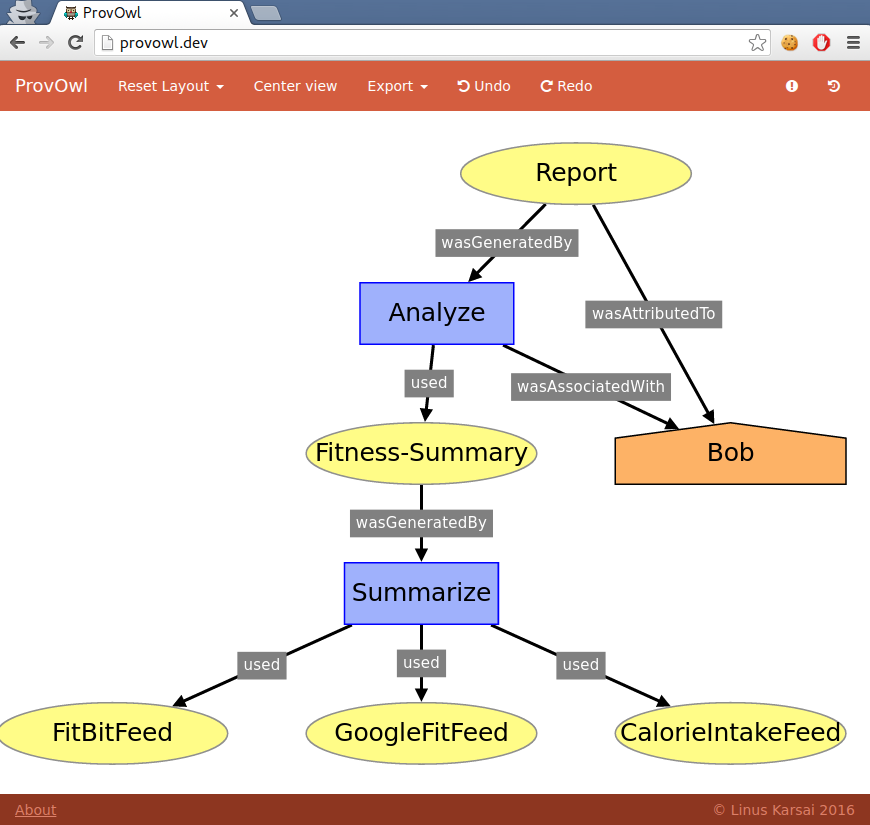
\includegraphics[width=\linewidth]{fitness-ungrouped}
	\caption{Provenance Data, as viewed in our \textit{ProvOwl} prototype. This labelled acyclic graph shows Bob's role in creating a report based on his fitness data. }
	\label{fig:fitness-ungrouped}
\end{figure}

\begin{figure}[h]
	\centering
	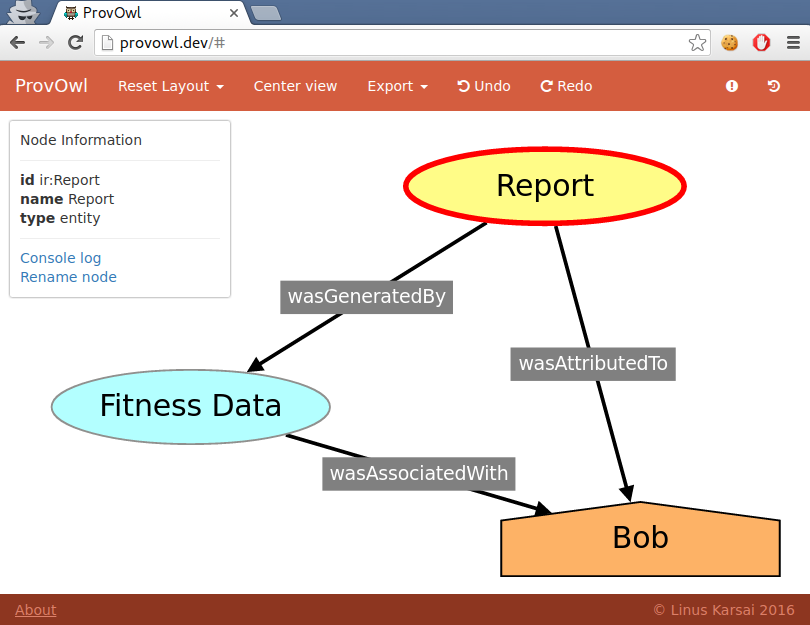
\includegraphics[width=\linewidth]{fitness-grouped}
	\caption{The graph of Fig.~\ref{fig:fitness-ungrouped}, after the user selected the \texttt{Analyze} node, with all its children, and clustered them, as a new node named \texttt{Fitness Data}. The user has selected the \texttt{Report} node, indicated by the red outline, and its details appear at the top left. Contextual actions are show in blue text in the details panel: \emph{Console log} is a debugging tool for printing the selected node to the console and \emph{Rename node} allows the user to change the name of the node. If multiple nodes where selected there would also be an option to group nodes.}
	\label{fig:fitness-grouped}
\end{figure}
